\documentclass[10pt, a4paper]{article}
\usepackage{hyperref}
\usepackage{graphicx}

\title{Simulating Free Fall: An Object Under Constant Gravitational acceleration}
\date{April 29, 2025}
\author{Matthew Coetzee}

\begin{document}

\maketitle

\section{Abstract}
The aim of this paper is to simulate objects in free fall. This will be done via simulation done in VS code using python. The data was recorded and shall be presented visually in graphs.

\section{Introduction}
This research paper aims to simulate and visualize the displacement and velocity of an object in free fall. Free fall is defined as the motion of an object under the influence of gravity alone. In the 1600s Galileo Galilei determined that all objects behave the same under free fall, regardless of mass and proportions. For the purposes of this paper, air resistance has not been simulated.

\section{Theory}
There are two equations that are important in simulating and understanding free fall. To understand free fall, we must know an object's velocity and displacement at any given time during the period of free fall. Displacement is determined via the following formula: 
$$s = \frac{1}{2}gt^2$$
In the above formula, $s$ is the displacement, $g$ is the gravitational constant ( $9.81 m/s^2$ on Earth), and $t$ represents the time that has elapsed.
Velocity is determined via the following formula:
$$v = gt$$
Where $v$ represents velocity, $g$ is again the gravitational constant, and $t$ is again the amount of time that has elapsed.
Here we can also note that Galileo’s observation is true. Two relevant formulas are:\\
Newtons Second Law: $$F = ma$$ and the force of gravity: $$F=mg$$ After rudimentary algebra we can observe that $m$ – the objects mass – cancels out, leaving acceleration to be equal to gravity, thus proving that gravity is independent from an objects mass (under true free fall).

\section{Method}
To simulate the motion of an object in free fall, I first wrote a basic python script in VS Code using python 3.13.3 (see addendum), that simulates and records the displacement and velocity of an object after a time-step of 0.1 seconds over 10 seconds, using the aforementioned formulas. I then proceeded to plot this data using the matplotlib python library, utilising the NumPy library to record the data in arrays that I used to plot two graphs. The plotted graphs compare displacement and velocity after certain points in time, respectively. It is here worth noting that no physical object was dropped, however all simulated results accurately matched expected results.

\section{Results}
After running the simulation, the following graphs were produced:
 
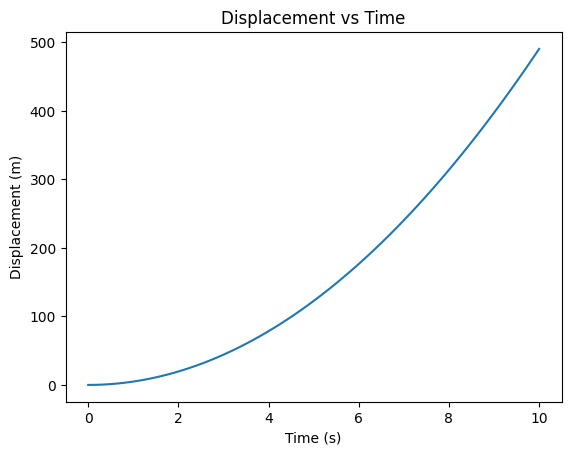
\includegraphics[scale=0.8]{DisVsTime}
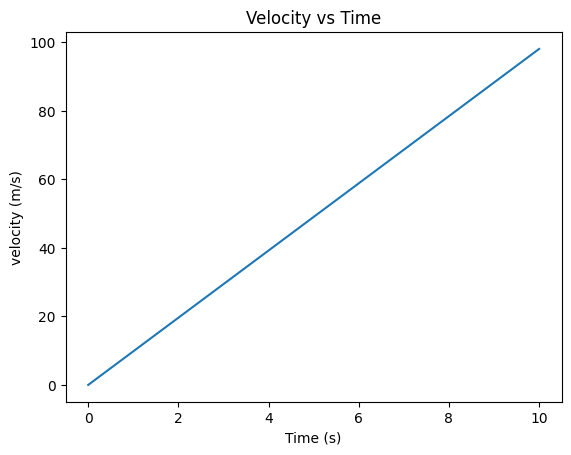
\includegraphics[scale=0.8]{VelVsTime}

\subsection{Displacement vs Time}
The first graph (on the left) compares displacement and time. You can observe that it is a quadratic function – noted by the porabola – where displacement is proportional to time squared. This observation aligns with the formula, in which time is squared.

\subsection{Velocity vs Time}
The second graph (on the right) compares velocity and time. Unlike the previous graph, this plot is linear where velocity and time directly scale with eachother. You can also note that the slope of this graph is equal to 9.81, which aligns with the equation for velocity in which the gravitational constant is equal to $9.81 ms^{-2}$. 

\subsection{How They Relate}
This tells us two things. Firstly that velocity undergoes constant acceleration and that an object falls further the longer it has been falling (again aligning with the formula, in which time is squared.)

\section{Discussion}
Saying this, it is again worth noting that mass and shape are not variables to be considered in true free fall, however if the two objects were dropped in an environment such as Earth, where air resistance is non-negligible, then the mass and shape of the objects are important factors to be considered. 
This aligns with recorded results, such as when Astronaut David Scott dropped a hammer and a feather on the lunar surface (implying no present atmosphere) during the Apollo 15 mission in 1971, when both objects fell at the same rate and came into contact with the ground at the same time.

\section{Conclusion}
This simulation successfully modelled the motion of an object in free fall under constant gravitational acceleration, assuming no air resistance. By applying the fundamental equations of motion, the results confirmed the expected behaviour: displacement increases quadratically over time, while velocity increases linearly.

These findings are consistent with both theoretical predictions and historical observations, such as Galileo’s experiments and the Apollo 15 demonstration on the Moon. Although simplified, the simulation effectively illustrates key concepts in kinematics and serves as a foundation for more complex models, such as those incorporating air resistance or varying gravitational environments.

\section{References}
ChatGPT, OpenAI. Physics Simulation Guidance 28 April 2025.

Personal Interview.\\
\\
\textit{NASA}. “Transcript of Apollo 15.” Ed. Eric M. Jones. n.d.

\url{https://www.nasa.gov/history/alsj/a15/a15.clsout3.html.}\\
\\
W3Schools. Python Matplotlib Tutorial. n.d. 

\url{https://www.w3schools.com/python/matplotlib_intro.asp.} 28 April 2025.



\end{document}